\documentclass[11pt,a4paper]{article}
\usepackage[spanish,es-nodecimaldot]{babel}	% Utilizar español
\usepackage[utf8]{inputenc}					% Caracteres UTF-8
\usepackage{graphicx}						% Imagenes

\PassOptionsToPackage{hyphens}{url}
\usepackage[hidelinks]{hyperref}			% Poner enlaces sin marcarlos en rojo

\usepackage{fancyhdr}						% Modificar encabezados y pies de pagina
\usepackage{float}							% Insertar figuras
\usepackage[textwidth=390pt]{geometry}		% Anchura de la pagina
\usepackage[nottoc]{tocbibind}				% Referencias (no incluir num pagina indice en Indice)
\usepackage{enumitem}						% Permitir enumerate con distintos simbolos
\usepackage[T1]{fontenc}					% Usar textsc en sections
\usepackage{amsmath}						% Símbolos matemáticos
\usepackage{listings}
\usepackage{algorithm}
\usepackage{amssymb}

% no accents in math operators
\unaccentedoperators

\usepackage{color}
 
\definecolor{codegreen}{rgb}{0,0.6,0}
\definecolor{codegray}{rgb}{0.5,0.5,0.5}
\definecolor{codepurple}{rgb}{0.58,0,0.82}
\definecolor{backcolour}{rgb}{0.95,0.95,0.92}
 
\lstdefinestyle{mystyle}{
    backgroundcolor=\color{backcolour},   
    commentstyle=\color{codegreen},
    keywordstyle=\color{magenta},
    numberstyle=\tiny\color{codegray},
    stringstyle=\color{codepurple},
    basicstyle=\footnotesize,
    breakatwhitespace=false,         
    breaklines=true,                 
    captionpos=b,                    
    keepspaces=true,                 
    numbers=left,                    
    numbersep=5pt,                  
    showspaces=false,                
    showstringspaces=false,
    showtabs=false,                  
    tabsize=2
}
 
\lstset{style=mystyle, language=Python}

% Comando para poner el nombre de la asignatura
\newcommand{\asignatura}{Visión por Computador}
\newcommand{\autor}{Vladislav Nikolov Vasilev}

% Configuracion de encabezados y pies de pagina
\pagestyle{fancy}
\lhead{Vladislav Nikolov, José María Sánchez}
\rhead{\asignatura{}}
\lfoot{Grado en Ingeniería Informática}
\cfoot{}
\rfoot{\thepage}
\renewcommand{\headrulewidth}{0.4pt}		% Linea cabeza de pagina
\renewcommand{\footrulewidth}{0.4pt}		% Linea pie de pagina

\begin{document}
\pagenumbering{gobble}

% Pagina de titulo
\begin{titlepage}

\begin{minipage}{\textwidth}

\centering

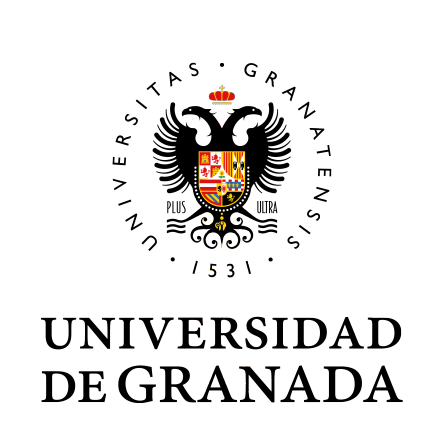
\includegraphics[scale=0.5]{img/ugr.png}\\

\textsc{\Large \asignatura{}\\[0.2cm]}
\textsc{GRADO EN INGENIERÍA INFORMÁTICA}\\[1cm]

\noindent\rule[-1ex]{\textwidth}{1pt}\\[1.5ex]
\textsc{{\Huge PROYECTO FINAL\\[0.5ex]}}
\noindent\rule[-1ex]{\textwidth}{2pt}\\[3.5ex]

\end{minipage}

\vspace{1cm}

\begin{minipage}{\textwidth}

\centering

\textbf{Autores}\\ {\autor{}}\\{José María Sánchez Guerrero}\\[2ex]
\textbf{Rama}\\ {Computación y Sistemas Inteligentes}\\[2ex]
\vspace{0.3cm}


\includegraphics[scale=0.3]{img/etsiit.jpeg}

\vspace{0.7cm}
\textsc{Escuela Técnica Superior de Ingenierías Informática y de Telecomunicación}\\
\vspace{1cm}
\textsc{Curso 2018-2019}
\end{minipage}
\end{titlepage}

\pagenumbering{arabic}
\tableofcontents
\thispagestyle{empty}				% No usar estilo en la pagina de indice


\newpage

\setlength{\parskip}{1em}

\section{\textsc{Descripción del problema}}

El problema que hemos escogido al alimón consiste en adaptar una red siamesa a un nuevo problema.
En este caso, vamos a adaptar una red preentrenada con imágenes de caras al problema de determinar
si dos personas están emparentadas o no a partir de fotos de sus caras. Este es un problema perfecto
para un tipo de red así, ya que normalmente redes de este tipo se utilizan en problemas de reconocimiento
facial (por ejemplo, determinar si dos fotos pertenecen o no a la misma persona). Por tanto, coger una red
de este tipo y aplicarla a un problema en el que también tenemos que comparar caras de personas
para determinar si están emparentadas parece lógico.

% Poner referencia a la pagina
El conjunto de datos con el que vamos a trabajar es el \textbf{\textit{Recognizing Faces in the Wild}},
creado por SMILE Lab de la Universidad de Northeastern, y contiene una serie de directorios los cuales
pertenecen a distintas familias. Cada una de estas familias está formada por uno o más individuos,
de los que se dispone de una o más fotos.

El conjunto de datos viene dividido en \textit{training} y test. El conjunto de entrenamiento sigue la estructura
anteriormente definida y viene acompañado de un archivo llamado ``\textit{train\_relationships.csv}'', el
cuál indica las relaciones de parentesco entre los individuos de las distintas familias (solo las relaciones
positivas). No obstante, el conjunto de test no sigue la estructura de directorios anteriormente descrita,
si no que vienen las imágenes sueltas acompañadas del archivo ``\textit{sample\_submission.csv}'', el cuál
indica las parejas de imágenes que se quiere verificar si son o no parientes.

% Decidir proporcion de validacion
En el conjunto de entrenamiento disponemos de unas 786 familias. En total tenemos unos 3965 individuos, y cada
familia está compuesta por un número variable de estos. Las imágenes que tenemos están a color y tienen un
tamaño de $224 \times 224$ píxeles. En total disponemos de 20726 imágenes de entrenamiento. No obstante, sería
interesante dejar una parte de las imágenes para validar el modelo, para ver cómo lo va haciendo con datos
que nunca antes a visto a medida que va entrenando. En secciones posteriores explicaremos cómo
hemos determinado con qué imágenes entrenar y cuántas imágenes serán de validación y cómo se irán generando.

El conjunto de test está formado por 4866 imágenes de las mismas características que las de entrenamiento.
Además, como hemos dicho anteriormente, disponemos de un archivo en formato \texttt{CSV} que indica
las parejas de imágenes para las que se quiere determinar si son parientes o no. Ya que disponemos de este
conjunto de datos, vamos a utilizarlo para ver cómo de bien lo hace nuestro modelo con imágenes nunca antes
vistas. Como no disponemos de las etiquetas reales, la forma de comprobar los resultados será rellenar el archivo
\texttt{CSV} anterior con las predicciones y subirlo a \textit{Kaggle}, donde en unos pocos segundos obtendremos
la \textit{accuracy} que hemos obtenido.

En cuanto a la salida, debido a la naturaleza del problema, la red va a obtener un valor entre 0 y 1.
El valor 0 representa que las dos personas no están emparentadas, mientras que el 1 representa que
están emparentadas. Los valores intermedios dirán que hay un determinado grado de parentesco entre
las dos personas. Como no disponemos de un valor umbral para determinar a partir del que podamos discernir
si dos personas están emparentadas o no, subiremos los resultados a \textit{Kaggle} y veremos cómo de buenos
han sido.

\section{\textsc{Enfoque elegido para el análisis}}

El análisis y el diseño del modelo y de nuestra red siamesa está formado por varias fases, las cuáles
detallaremos a continuación:

\begin{itemize}
    \item red usada
    \item Primero leeremos y preprocesaremos los datos
    \item Generar los datos a utilizar (train y validación)
        
        \begin{itemize}
            \item Batch generator
            \item Data generator
        \end{itemize}
        
        Comentar también el dataset to images
    \item Diseño y entrenamiento de la red siamesa y resultados obtenidos
    \item Mejora de la red por defecto
\end{itemize}

\section{\textsc{Red}}

\section{\textsc{Lectura y procesamiento de datos}}

En esta sección vamos a ver cómo leemos los datos de entrada y como los preprocesamos para poder trabajar con
ellos de una forma más cómoda. Lo primero que haremos será pasar la ruta donde tenemos guardado nuestro
\textit{dataset} a una función, y a partir de ella, obtendremos una lista con todos los miembros de cada familia
y un diccionario con las rutas de las imágenes disponibles de cada individuo. La función que nos permite esto
es la siguiente:

\begin{lstlisting}
def read_family_members_images(data_path):
    """
    Funcion que procesa la ruta especificada como parametro. Obtiene
    una lista con los miembros de cada familia, la cual tendra el
    formato "FXXXX/MIDY", y un diccionario con las rutas de las
    imagenes de cada miembro de cada familia.

    Args:
        data_path: Ruta de los archivos a procesar.
    
    Return:
        Devuelve una lista con los miembros de cada familia y un
        diccionario con las imagenes de cada miembro de cada familia.
    """
    # Leer la ruta proporcionada y obtener todos los directorios
    # Cada directorio esta asociado a una familia
    dirs = sorted(list(glob.glob(data_path + "*")))

    # Obtener los nombres de los directorios de las familias
    family_dirs = np.array([dir.split("/")[-1] for dir in dirs])

    # Obtener imagenes asociadas a cada directorio
    images = {f"{family}/{member.split('/')[-1]}": sorted(list(glob.glob(member + "/*.jpg")))
        for family in family_dirs for member in sorted(list(glob.glob(f"{data_path}{family}/*")))
    }
    
    family_members_list = list(images.keys())
    
    return family_members_list, images
\end{lstlisting}

Una vez disponemos de las rutas de las imágenes, ahora tendremos que leerlas. Para ello utilizamos una función a
la cual le pasamos una de las rutas obtenidas y nos cargará la imagen como un array de números reales. Posteriormente,
preprocesamos la imagen gracias a una función del modelo \textit{keras-vggface}[referencia al modelo] diseñada especialmente
para esta implementación.

\begin{lstlisting}
def read_image(path):
    """
    Funcion que permite leer imagenes a partir de un archivo
    Args:
        path: Ruta de la imagen
    """
    img = cv2.imread(path)
    img = np.array(img).astype(np.float)
    return preprocess_input(img, version=2)
\end{lstlisting}

Podemos ver en la función de preprocesado que tenemos un parámetro '\textit{version}'. Este parámetro habrá que establecerlo,
como nos dice el propio autor, en 1 para \textit{VGG16} o en 2 para \textit{RESNET50} o \textit{SENET50}.


\section{\textsc{División y generación de datos}}

Una vez que hemos leído los datos y hemos generado la lista de individuos y el diccionario
que permite acceder a las imágenes de cada individuo, vamos a dividir la lista de individuos
que tenemos en dos conjuntos.

Por un lado tendremos el conjunto de entrenamiento, donde tendremos aquellos individuos que
podremos combinar entre ellos para entrenar la red. Por otro lado, tendremos el conjunto de
validación, donde tendremos


\begin{lstlisting}
def generate_datasets(families, val_prop=0.2):
    """
    Funcion que permite generar los datasets de train, test y
    validacion a partir de un array de directorios, los cuales
    representan las familias. Los datos son mezclados para que
    se escoja de forma aleatoria.

    Args:
        families: Array con los directorios de las familias.
        test_prop: Proporcion de los datos totales que tiene
                   que estar en el conjunto de test.
        val_prop: Proporcion de los (datos_totales - datos_test)
                  que tienen que estar en el conjunto de validacion.
    
    Return:
        Devuelve un array con los directorios de las familias que
        forman el conjunto de train, otro para el conjunto de
        validacion y otro para el conjunto de test.
    """
    # Mezclar familias
    shuffle_families = np.copy(families)
    np.random.shuffle(shuffle_families)

    # Obtener la ultima proporcion de las familias y guardarla en
    # el conjunto de validacion
    idx_val = int(len(shuffle_families) * (1 - val_prop))
    val_dirs = shuffle_families[idx_val:]
    train_dirs = shuffle_families[:idx_val]

    # Volver a mezclar familias del conjunto de entrenamiento
    np.random.shuffle(train_dirs)

    return train_dirs, val_dirs
\end{lstlisting}

Debido a que el número de parejas de imágenes que se pueden formar es del orden de cientos de millones
y a que tenemos restricciones muy fuertes sobre el \textit{hardware} y el tiempo de los que disponemos,
no nos podemos permitir entrenar y validar el modelo con cada posible pareja. Por tanto, tenemos
que encontrar una forma de 


\subsection{\textit{Batch Generator}}


\begin{lstlisting}
def batch_generator(dataset, images, relationships_path,
                    batch_size=32, relationships_prop=0.2):
    """
    Funcion que selecciona aleatoriamente dos conjunto de individuos
    y sus etiquetas, asigna una proporcion de parejas con parentesco
    entre los dos conjuntos, y devuelve en cada iteracion la
    cantidad asignada como tamanio de batch.
    Args:
        dataset: Array con los directorios de las familias.
        images: Array con los directorios de las imagenes de cada
                individuo de la familia.
        relationships_path: Ruta del archivo de relaciones a procesar.
        batch_size: Tamanio del batch.
        relationships_prop: Proporcion de individuos con un parentesco
                            familiar tendran los datos generados.
    
    Return:
        Devuelve dos arrays con los individuos que seran procesados
        por cada una de las partes de nuestra red, y un array con los
        parentescos entre los arrays anteriores
    """
    # Leemos el archivo donde se encuentran las relaciones familiares
    # entre individuos
    relationships = pd.read_csv(relationships_path)
    relationships = list(zip(relationships.p1.values,
                             relationships.p2.values))
    
    while True:
        # Generamos un conjunto de imagenes aleatorias y lo devolvemos
        # hasta que el iterador vuelva a pedir otro
        left_images, right_images, targets = dataset_to_images(dataset, images, relationships, batch_size, relationships_prop)

        yield [left_images, right_images], targets
\end{lstlisting}



\subsection{\textit{Data Generator}}

\begin{lstlisting}
    def data_generator(dataset, images, relationships_path,
                       data_size, relationships_prop=0.2):
    """
    Funcion que selecciona aleatoriamente dos conjunto de individuos
    y sus etiquetas, asigna una proporcion de parejas con parentesco
    entre los dos conjuntos, y los devuelve.
    Args:
        dataset: Array con los directorios de las familias.
        images: Array con los directorios de las imagenes de cada
                individuo de la familia.
        relationships_path: Ruta del archivo de relaciones a procesar.
        data_size: Tamanio de los datos a generar.
        relationships_prop: Proporcion de individuos con un parentesco
                            familiar que tendran los datos generados.
    
    Return:
        Devuelve dos arrays con los individuos que seran procesados
        por cada una de las partes de nuestra red, y un array con los
        parentescos entre los arrays anteriores
    """
    # Leemos el archivo donde se encuentran las relaciones familiares
    # entre individuos
    relationships = pd.read_csv(relationships_path)
    relationships = list(zip(relationships.p1.values,
                             relationships.p2.values))

    # Generamos un conjunto de imagenes aleatorias y las devolvemos
    left_images, right_images, targets = dataset_to_images(dataset, images, relationships, data_size, relationships_prop)

    return [left_images, right_images], targets
\end{lstlisting}







\section{Generación de resultados}

\begin{lstlisting}
test_path = "content/test/"
submission = pd.read_csv("content/sample_submission.csv")

predictions = []

for batch in submission.img_pair.values:
    X1 = [x.split("-")[0] for x in batch]
    X1 = np.array([read_image(test_path + x) for x in X1])

    X2 = [x.split("-")[1] for x in batch]
    X2 = np.array([read_image(test_path + x) for x in X2])

    pred = model.predict([X1, X2]).ravel().tolist()
    predictions += pred

submission['is_related'] = predictions
submission.to_csv("drive/My Drive/Proyecto/vgg_face-regularizers.csv", index=False)
\end{lstlisting}


\section{\textsc{Elección y diseño de la red}}
Diseño inicial
Sin las densas finales, capas no entrenables y Adam por defecto (0.6 prop)
    - Resnet50
    - Senet50
    - Vggface

\section{Mejora de la red implementada}

Condiciones: 30 épocas, 100 pasos train, 30 validación y capas entrenables

Cambiando Adam bajando lr
Metiendo densas finales
RMSProp
Focal loss
Regularizers <- el bueno
%Subiendo a 0.8
%Subiendo a 0.8 validacion
% Volver con densas a 0.6






\end{document}
